\documentclass[a4paper,11pt,twoside,openright]{report}

\usepackage{graphicx}
%\usepackage{ngerman}
\usepackage[utf8x]{inputenc}
\usepackage{fancyvrb}
\usepackage{courier}
\usepackage{helvet}
\usepackage{tikz}
\usepackage{xcolor}
\usepackage{pdfpages}
\usepackage[strict]{changepage}
\usepackage{xspace}

\pdfoptionpdfminorversion=6

% \definecolor{se_dark_blue}{RGB}{0,103,166} % powerpoint
\definecolor{se_dark_blue}{RGB}{0,96,178} % website
% \definecolor{se_light_blue}{RGB}{119,158,201} % powerpoint
\definecolor{se_light_blue}{RGB}{129,160,225} % website


%% setup listings
\usepackage{listings}
\lstset{
    numbers=left,
    numberstyle=\tiny,
    numbersep=5pt,
    xleftmargin=11pt,
    xrightmargin=4pt,
    frame=single,
    aboveskip=0pt,
    belowskip=-6pt,
    sensitive=true,
    float=!t,
    breaklines=false,
    captionpos=b,
    tabsize=2,
    showstringspaces=false,
    basicstyle=\small\ttfamily,
    morecomment=[l]{//},
    morecomment=[s][\itshape]{/**}{*/}
}

%% defines the listings laguage named 'MontiArc' derived from the language 'Java' 
%% adding the below listed keywords. See 
%% ftp://ftp.tex.ac.uk/tex-archive/macros/latex/contrib/listings/listings.pdf
%% for listings documentation
\lstdefinelanguage{MontiArc}[]{Java}{
  morekeywords={component, port, in, out, inv, package, import, connect, autoconnect}
}

% Seite einrichten
\setlength{\voffset}{-1in}
\setlength{\hoffset}{-1in}

\setlength{\topmargin}{2.5cm}		   
\setlength{\headheight}{0cm}		   
\setlength{\headsep}{0cm}		   
\setlength{\oddsidemargin}{3,3cm}  % innen ein wenig mehr Rand für die Klebebindung
\setlength{\evensidemargin}{2,7cm} % dafür außen ein wenig weniger
\setlength{\textwidth}{15cm}		   
\setlength{\textheight}{23,5cm}		   
\setlength{\parindent}{0cm}

\newcommand{\emptyLine}{{\LARGE ~\\}}
\newcommand{\MontiCar}{MontiCar\xspace}


\begin{document}

% Einrücken von Absätzen verhindern und 1.5 Zeilen Absatzabstand
\setlength{\parindent}{0pt}
\setlength{\parskip}{1.5ex plus0.5ex minus0.5ex}

%% Dieses Teildokument beschreibt die Titelseite.
%

% Seitenzähler auf 1, Römische Ziffern.
\setcounter{page}{1}
\pagenumbering{roman}

\thispagestyle{headings}

%\changepage{<text height>}{<text width>}{<even-side margin>}{<odd-side margin>}{<column sep.>}{<topmargin>}{<headheight>}{<headsep>}{<footskip>}
\changepage{5,1cm}{2.4cm}{}{-0.7cm}{}{-2,3cm}{}{}{}

% Eigentliche Titelseite.
\begin{titlepage}
	
\begin{figure}\raggedleft
\includegraphics[height=3.0cm]{src/pic/logo.jpg}\end{figure}
  
\begin{tikzpicture}[overlay]

% horizontal lines
\draw[color=se_dark_blue, thick] (-1.6, 0.9) -- (17.4, 0.9);
\draw[color=se_light_blue, thick] (-1.4, 0.7) -- (17.4, 0.7);

% vertical lines
\draw[color=se_dark_blue, thick] (-1, 0.9) -- (-1, -24.5);
\draw[color=se_light_blue, thick] (-0.8, 0.7) -- (-0.8, -24.5);

\end{tikzpicture}

\vspace*{-1.5em}

\begin{flushleft}
  {\fontfamily{phv}  
  	{\LARGE
      Rheinisch Westfälische Technische Hochschule Aachen \\
      Lehrstuhl für Software Engineering \\}
    \vspace{3em}
  
    {\LARGE \textbf{Erste Titel-Zeile}\\} 
    {\LARGE \textbf{Zweite Titel-Zeile}\\} 
    {\LARGE \textbf{Dritte Titel-Zeile}\\} % Oder \emptyLine falls nicht Titel kürzer
    {\LARGE \textbf{Vierte Titel-Zeile}\\} % Oder \emptyLine falls nicht Titel kürzer
    \vspace{3em}
		
    {\Large \textbf{Diplomarbeit/Masterarbeit/Studienarbeit}\\}
		\vspace{3em} 
		
		{\large von\\} % presented by
    
    {\LARGE \textbf{Name, Vorname}\\}
    \vspace{3em} 
		    
    {\Large \textbf{1. Prüfer: Prof.\ Dr.\ B.\ Rumpe}\\}
    \vspace{1em} 
    {\Large \textbf{2. Prüfer: }\\}
    \vspace{1em} 
    {\Large \textbf{Betreuer: }\\}
    \vspace{7em} 

    {\large Diese Arbeit wurde vorgelegt am Lehrstuhl für Software Engineering \\}
    \vspace{1em}
    % The present work was submitted to the chair of software engineering
		{\large	Aachen, den \today\\}
  }
\end{flushleft}

\end{titlepage}

\changepage{-5,1cm}{-2.4cm}{}{0.7cm}{}{2,3cm}{}{}{}





 %Dieses Teildokument beschreibt die Titelseite.
%

% Seitenzähler auf 1, Römische Ziffern.
\setcounter{page}{1}
\pagenumbering{roman}

\thispagestyle{headings}

%\changepage{<text height>}{<text width>}{<even-side margin>}{<odd-side margin>}{<column sep.>}{<topmargin>}{<headheight>}{<headsep>}{<footskip>}
\changepage{5,1cm}{2.4cm}{}{-0.7cm}{}{-2,3cm}{}{}{}

% Eigentliche Titelseite.
\begin{titlepage}
	
\begin{figure}\raggedleft
\includegraphics[height=3.0cm]{src/pic/logo.jpg}\end{figure}
  
\begin{tikzpicture}[overlay]

% horizontal lines
\draw[color=se_dark_blue, thick] (-1.6, 0.9) -- (17.4, 0.9);
\draw[color=se_light_blue, thick] (-1.4, 0.7) -- (17.4, 0.7);

% vertical lines
\draw[color=se_dark_blue, thick] (-1, 0.9) -- (-1, -24.5);
\draw[color=se_light_blue, thick] (-0.8, 0.7) -- (-0.8, -24.5);

\end{tikzpicture}

\vspace*{-1.5em}

\begin{flushleft}
  {\fontfamily{phv}  
  	{\LARGE
      RWTH Aachen University \\
      Software Engineering Group \\}
    \vspace{3em}
  
    {\LARGE \textbf{Deep Learning in Autonomous Driving}\\} 
    {\LARGE \textbf{Direct Perception Approach}\\} 
    {\LARGE \textbf{ }\\} % Replace with \emptyLine if title is shorter
    {\LARGE \textbf{ }\\} % Replace with \emptyLine if title is shorter
    \vspace{3em}
		
    {\Large \textbf{Seminar Paper}\\}
		\vspace{3em} 
		
		{\large presented by\\} 
    
    {\LARGE \textbf{Bergerbusch, Timo}\\}
    \vspace{3em} 
		    
    {\Large \textbf{1st Examiner: Prof.\ Dr.\ B.\ Rumpe}\\}
    \vspace{1em} 
%    {\Large \textbf{2nd Examiner: }\\}
%    \vspace{1em} 
    {\Large \textbf{Advisor: Evgeny Kusmenko}\\}
    \vspace{7em} 

    {\large The present work was submitted to the Chair of Software Engineering \\}
    \vspace{1em}
    % The present work was submitted to the chair of software engineering
		{\large	Aachen, \today\\}
  }
\end{flushleft}

\end{titlepage}

\changepage{-5,1cm}{-2.4cm}{}{0.7cm}{}{2,3cm}{}{}{}




 % English cover

\clearpage

% Erklaerung

%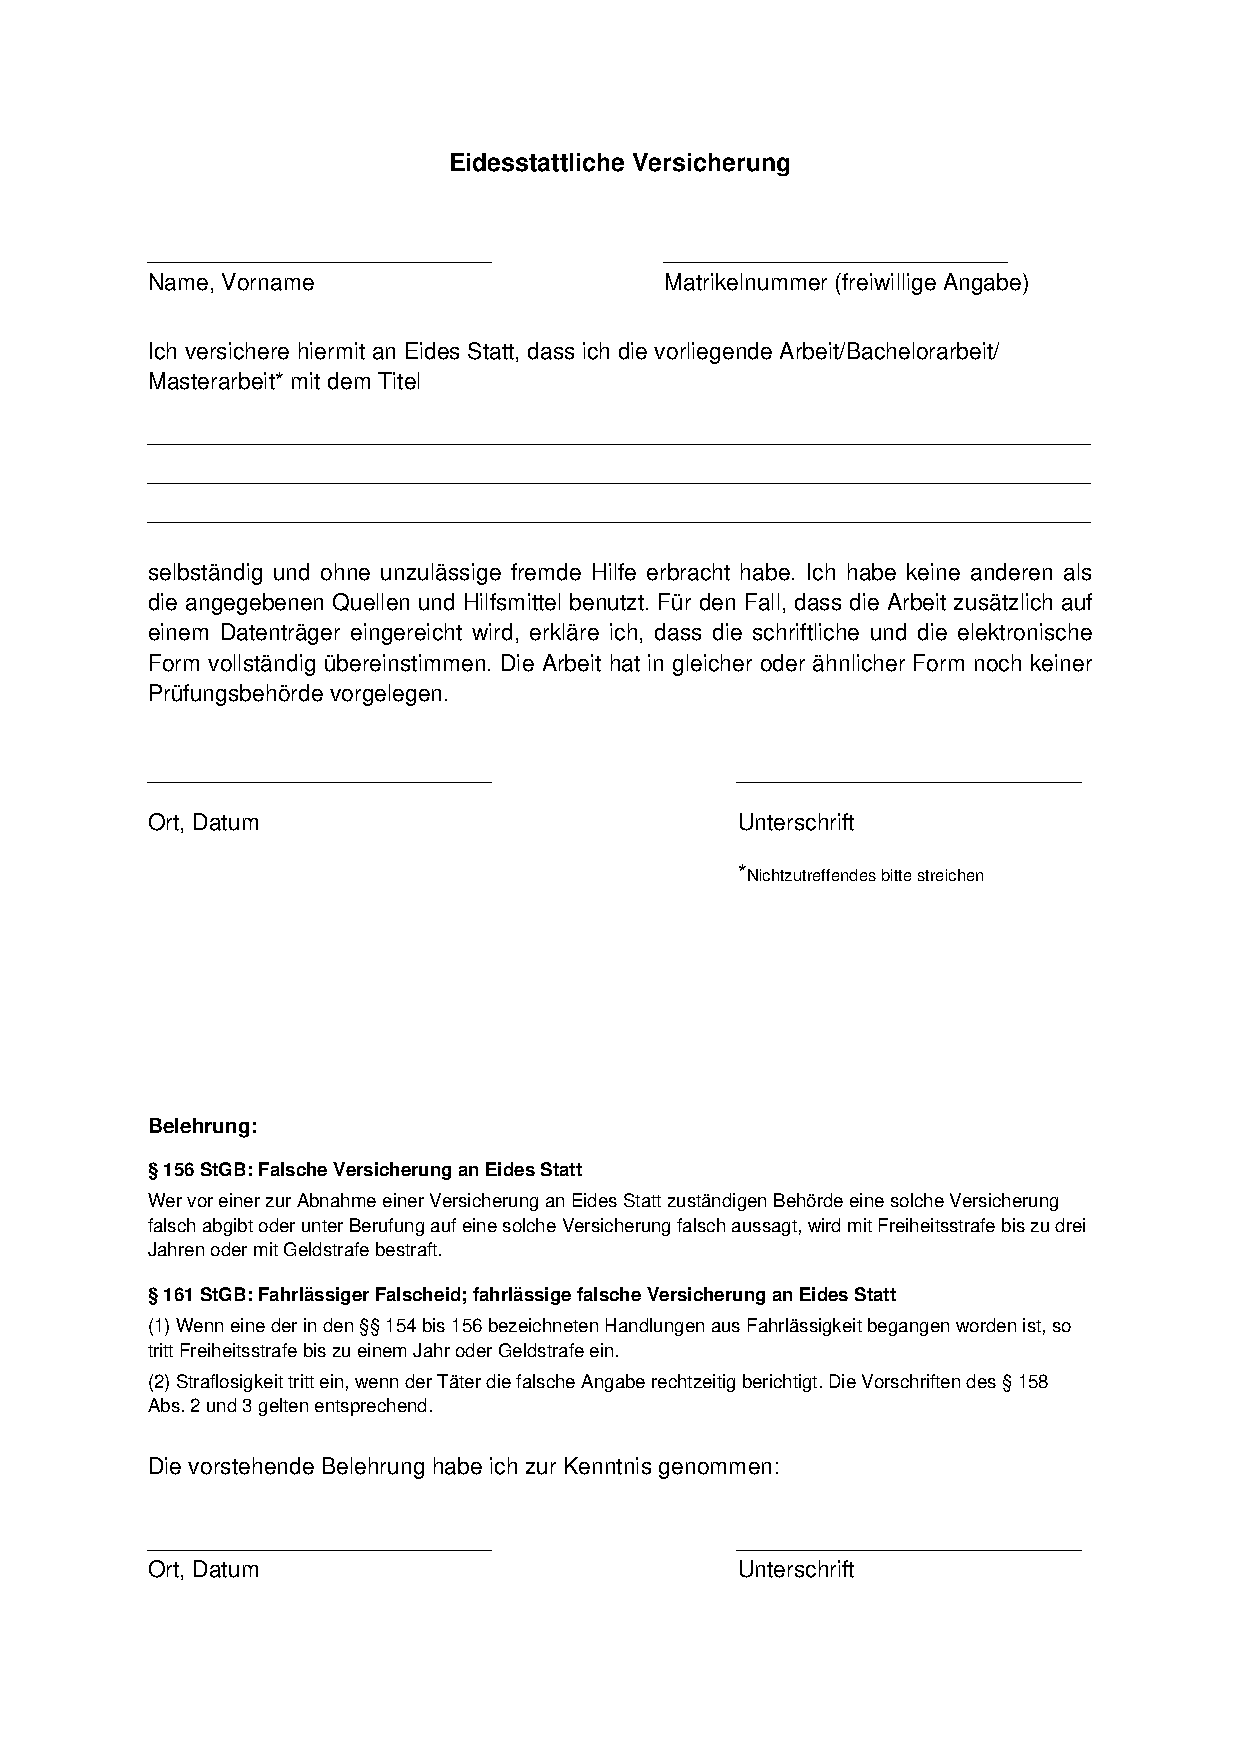
\includepdf[pages={1},offset=-1in -1in]{Formular_Eidesstattliche_Versicherung_neu.pdf}
 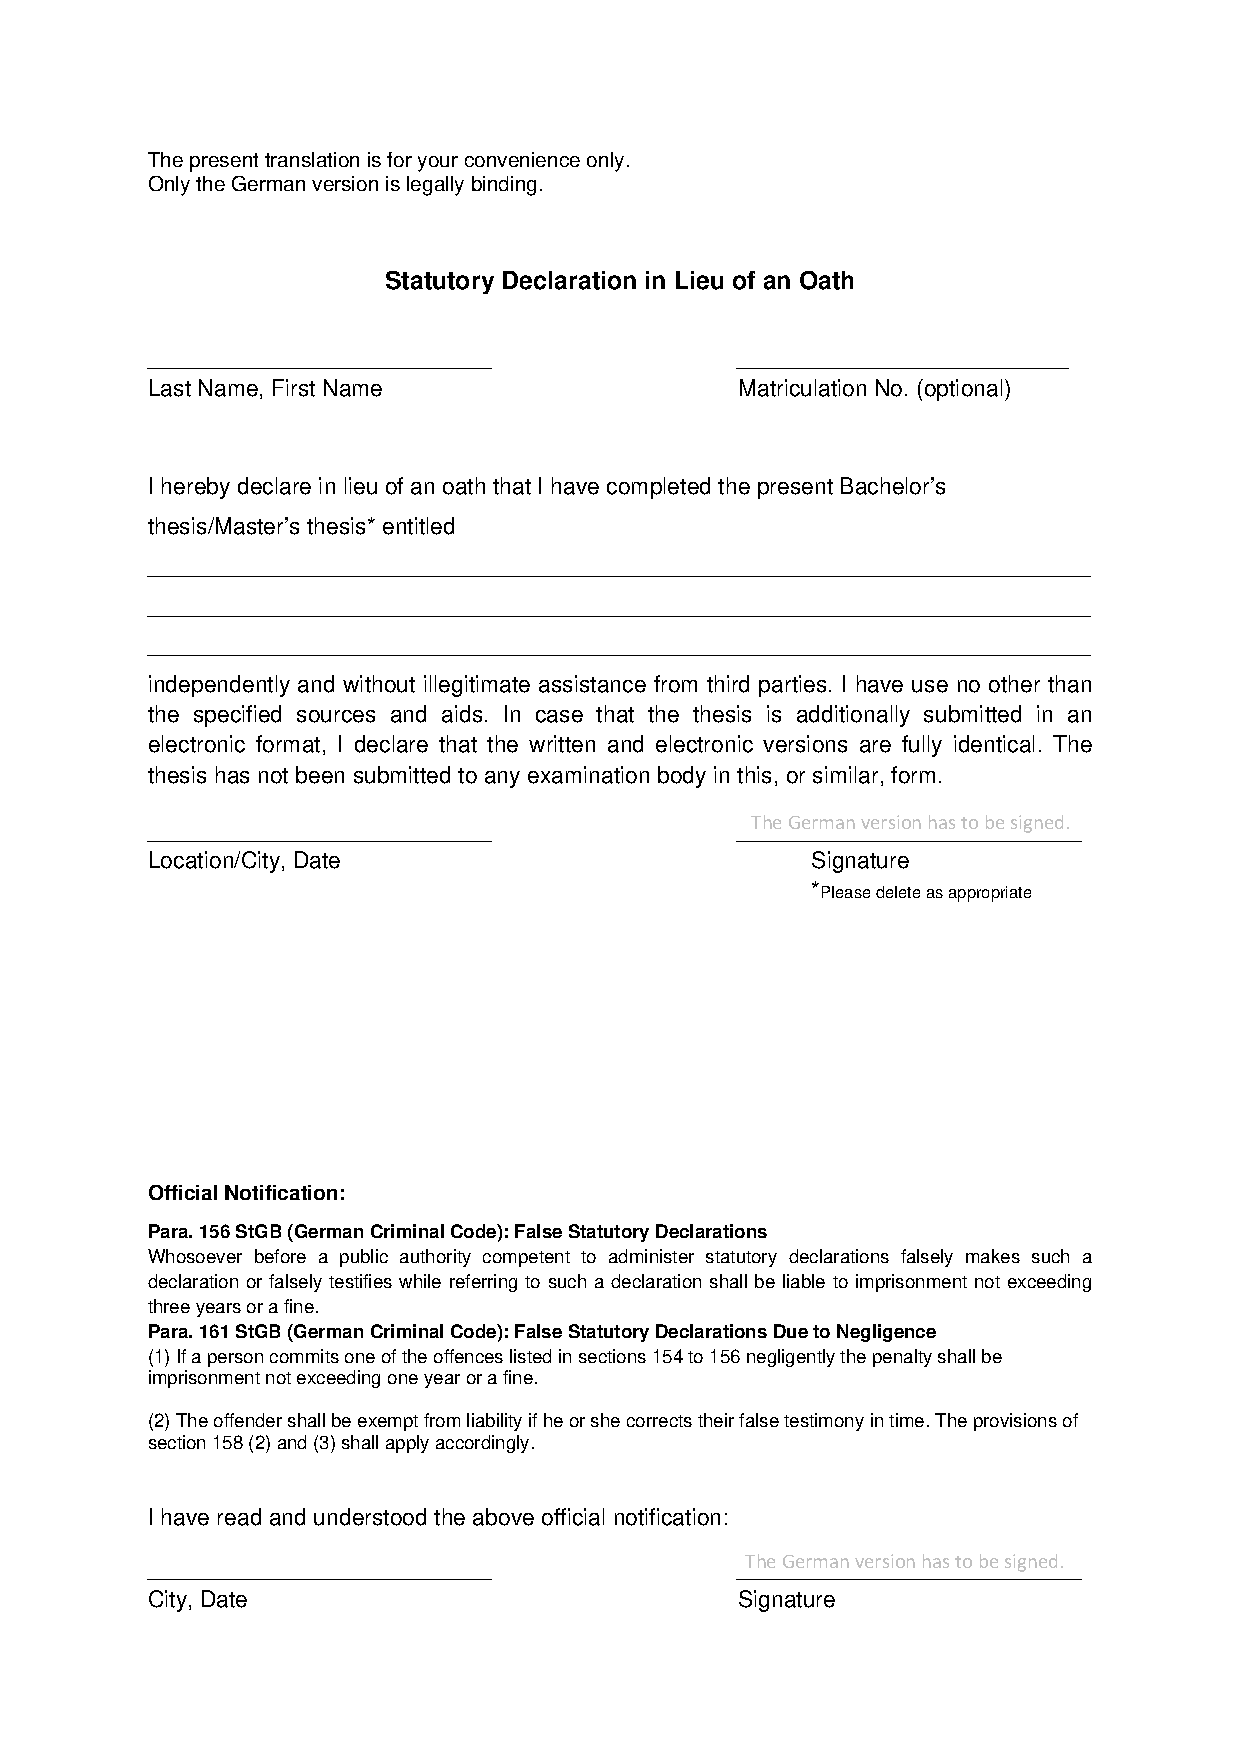
\includepdf[pages={1},offset=-1in -1in]{Statutory_Declaration_in_Lieu_of_an_Oath.pdf} % English 

\clearpage

%TODO rewrite
{\bf\Large Abstract} \\ [1em]
The topic of autonomous driving using artificial intelligence increases in importance with the overwhelming amount of software usage within vehicles. For that \textit{Convolutional Neural Networks} (CNNs), which try to figure out the importance of special areas of a single picture, have been shown to be promising. \\
In this paper we will give a general introduction to the topic of \nns and then state the specialties defining a CNN.
We distinguish between the three main paradigms currently used and researched for autonomous driving agents: mediated perception, behavior reflex and direct perception.\\
Further we will compare different domain specific languages \cnnarch, \caffe, \caffetwo and \mxnet, based on the factors of usability, scope of functionality, also regarding training possibilities, and the integration on a subject.

We will analyze a CNN using the direct perception approach, in different languages, and compare it to state-of-the-art implementations of the other paradigms, training on a simulator \torcs or the \kitti database. Furthermore we state scenarios probably causing problems for the direct perception approach. 

Finally we create an overview of the mentioned languages with a table, which states the functionalities and properties in a nutshell.
\cleardoublepage


\vspace*{2cm}
{\bf\Large Aufgabenstellung}

\cleardoublepage


\tableofcontents

\clearpage

% Ab erstem Kapitel Seiten arabisch zählen
\setcounter{page}{1}
\pagenumbering{arabic}

\chapter{Introduction}



\chapter{Simulators}
Introduce the different simulators choosen

\section{\MontiCar}
\section{Simulator 2}
\section{Simulator 3}

\section{General Comparison}





\chapter{Cooperative Behaviour}
Define the keyword "cooperative" and a set of essential assets a cooperative agent must have



\chapter{Testing}
Test the running example by simulating in simulators

\section{Implementation}

\section{Comparison}




%\chapter{Code Listings}\label{ch:listings}
%% use language 'myLng' for the next listings (until another language is set)
%% include listing 'listings/AdverseReactionApp.aj' with label and caption
%% note: big listings sometimes need to overwrite the float value that has been
%% already set in the general listings setup (see paper.tex)

This chapter contains the beautiful listing \ref{lst:system}. 
Lorem ipsum dolor sit amet, consetetur sadipscing elitr, sed diam nonumy 
eirmod tempor invidunt ut labore et dolore magna aliquyam erat, sed diam 
voluptua. At vero eos et accusam et justo duo dolores et ea rebum. Stet 
clita kasd gubergren, no sea takimata sanctus est Lorem ipsum dolor sit 
amet. Lorem ipsum dolor sit amet, consetetur sadipscing elitr, sed diam 
nonumy eirmod tempor invidunt ut labore et dolore magna aliquyam erat, 
sed diam voluptua. At vero eos et accusam et justo duo dolores et ea 
rebum. Stet clita kasd gubergren, no sea takimata sanctus est Lorem 
ipsum dolor sit amet. 




\begin{figure}[hbt]
\lstset{language=MontiArc}
\lstinputlisting[
label=lst:system,
caption=Code listing with user defined syntax highlighting (MontiArc).] {src/listings/AdverseReactionApp.aj}
\end{figure}

\cleardoublepage


\chapter{Conclusion}

Conclusion of differences and similarities between the frameworks\\

\begin{tabular}{l |c |c |c |c }
	Property 						& \cnnarch 		& \caffe 		& \caffetwo 		& \mxnet \\ \hline
					\multicolumn{5}{c}{General Information}\\\hline
	is full framework  				& \xmark		& \cmark		& \cmark			& \cmark \\
	SLI usage						& -- 			& \xmark$^1$ 	& \xmark$^1$ 		& \cmark \\
	mult. computers 				& -- 			& \cmark		& \cmark			& \cmark \\	
	\hline
					\multicolumn{5}{c}{Nets Supported}\\ \hline
	typical CNNs					& \cmark		& \cmark		& \cmark			& \cmark \\
	arbitrary CNNs					& \xmark		& \cmark		& \cmark			& \cmark \\
	Recurrent NNs					& \xmark		& \cmark		& \cmark			& \cmark \\
	\hline
					\multicolumn{5}{c}{Constructs}\\ \hline
	predefined NNs					& \cmark		& \cmark		& \cmark			& \cmark \\
	pretrained NNs  				& \xmark		& \cmark		& \xmark$^2$		& \cmark \\
	simple arbitrary net creation	& \cmark		& \xmark 		& \xmark			& \cmark \\	
	predefined functions 		  	& \cmark		& \cmark		& \cmark			& \cmark \\
	simple function creation 	  	& \cmark 		& \xmark		& \xmark$^2$		& \cmark \\
	low-level operations			& \xmark		& \xmark		& \xmark			& \cmark \\ %check
	\hline
					\multicolumn{5}{c}{Language bindings}\\ \hline
	C++								& \xmark		& \cmark		& \cmark			& \cmark \\
	Python							& \cmark		& \xmark$^3$	& \cmark			& \cmark \\
	MatLab							& ? 			& \cmark		& \xmark			& \cmark \\ 
	Others							& ?				& ?				& ?					& R, Go, Julia, Perl\\
									&				&				&					& JavaScript, Scala \\ 
%	\hline
%					\multicolumn{5}{c}{Usage}\\ \hline
%					understandability & & & & \\
%					handling & & & & \\
\end{tabular}

\begin{itemize}
	\item[$^1$] depending on CUDA version/installation
	\item[$^2$] not clearly stated, but also not denied
	\item[$^3$] added lately
\end{itemize}

Possible Criteria%SEE: 4.4.1 in CNNArchLang
\begin{itemize}
	\item generality
	\item expressiveness
	\item modularity
	\item is Framework?
	\item Installation 
	\item Error Handling
	\item for equal task?
	\item low-level computations
\end{itemize}
Also a general conclusion based on results and \cite{grzywaczewski2017training}

\bibliographystyle{alpha}
\addcontentsline{toc}{chapter}{Literaturverzeichnis}
\bibliography{src/bib/Literatur}

% Begin Anhang
%\appendix
%\chapter{z.\,B. Programmdokumentation}

\cleardoublepage


\end{document}
